\documentclass{standalone}
\usepackage{tikz}
\usetikzlibrary{arrows,calc,decorations.pathreplacing,positioning}

\tikzset{
    state/.style={
        circle,
        minimum width=1cm,
        inner sep=0pt,
        text centered,
        draw,
    },
    stateObs/.style={
        state,
        minimum width=2cm,
    },
    obs/.style={
        rectangle,
        minimum width=1cm,
        text centered,
        draw,
    },
    obsState/.style={
        obs,
        minimum width=2cm,
    },
    line/.style={
        very thick,
        -latex',
    }
}

\begin{document}
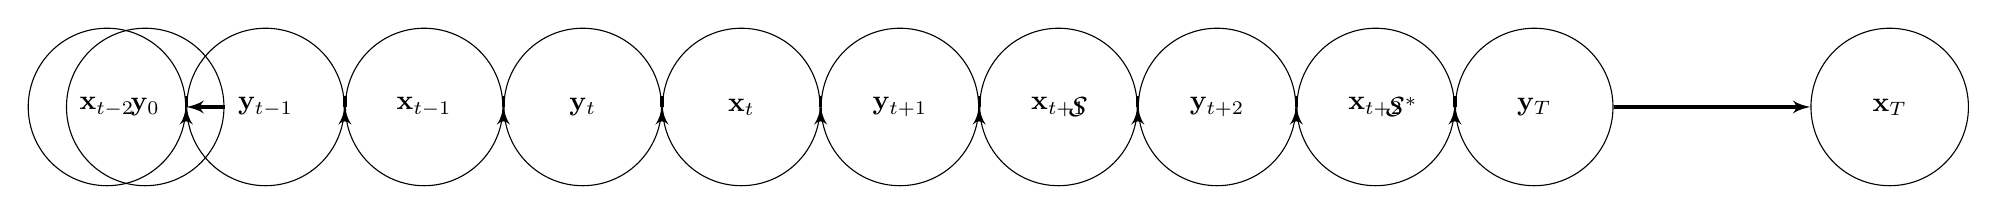
\begin{tikzpicture}[node distance=0mm]
\node[stateObs](X0){$\mathbf{y}_0$};
\node[stateObs,right=of X0,xshift=-2.5cm](X1){$\mathbf{x}_{t-2}$};
\node[stateObs,right=of X1](X2){$\mathbf{y}_{t-1}$};
\node[stateObs,right=of X2](X3){$\mathbf{x}_{t-1}$};
\node[stateObs,right=of X3](X4){$\mathbf{y}_t$};
\node[stateObs,right=of X4](X5){$\mathbf{x}_{t}$};
\node[stateObs,right=of X5](X6){$\mathbf{y}_{t+1}$};
\node[stateObs,right=of X6](X7){$\mathbf{x}_{t+1}$};
\node[stateObs,right=of X7](X8){$\mathbf{y}_{t+2}$};
\node[stateObs,right=of X8](X9){$\mathbf{x}_{t+2}$};
\node[stateObs,right=of X9](X10){$\mathbf{y}_{T}$};

\node[stateObs,right=of X10,xshift=2.5cm](X11){$\mathbf{x}_T$};

\draw[line](X0)--(X1);
\draw[line](X1)--(X2);
\draw[line](X2)--(X3);
\draw[line](X3)--(X4);
\draw[line](X4)--(X5);
\draw[line](X5)--(X6);
\draw[line](X6)--(X7);
\draw[line](X7)--(X8);
\draw[line](X8)--(X9);
\draw[line](X9)--(X10);
\draw[line](X10)--(X11);

\path[dotted] ($(X2.north west)!0.5!(X3.south east)$)rectangle($(X7.north west)!0.5!(X8.south east)$);
\path[dashed] ($(X1.south west)!0.5!(X4.north east)$)rectangle($(X9.south west)!0.5!(X10.north east)$);
\node[right=1cm of X7,xshift=-2cm,font=\itshape]{$\mathcal S$};
\node[right=1cm of X9,xshift=-2cm,font=\itshape]{$\mathcal S^*$};
\end{tikzpicture}
\end{document}